\documentclass{standalone}
\usepackage{tikz}
\usetikzlibrary{positioning, arrows.meta}

% Define styles for nodes and edges
\tikzset{
    place/.style={
        circle,
        draw=black,
        fill=white,
        minimum size=7mm,
        inner sep=0pt,
        outer sep=0pt,
    },
    transition/.style={
        rectangle,
        draw=black,
        fill=gray!50,
        minimum width=7mm,
        minimum height=7mm,
        inner sep=0pt,
        outer sep=0pt,
    },
    arrow/.style={
        ->,
        >=Stealth,
        thick,
    },
    label/.style={
        font=\footnotesize,
        align=center,
    },
}

\begin{document}

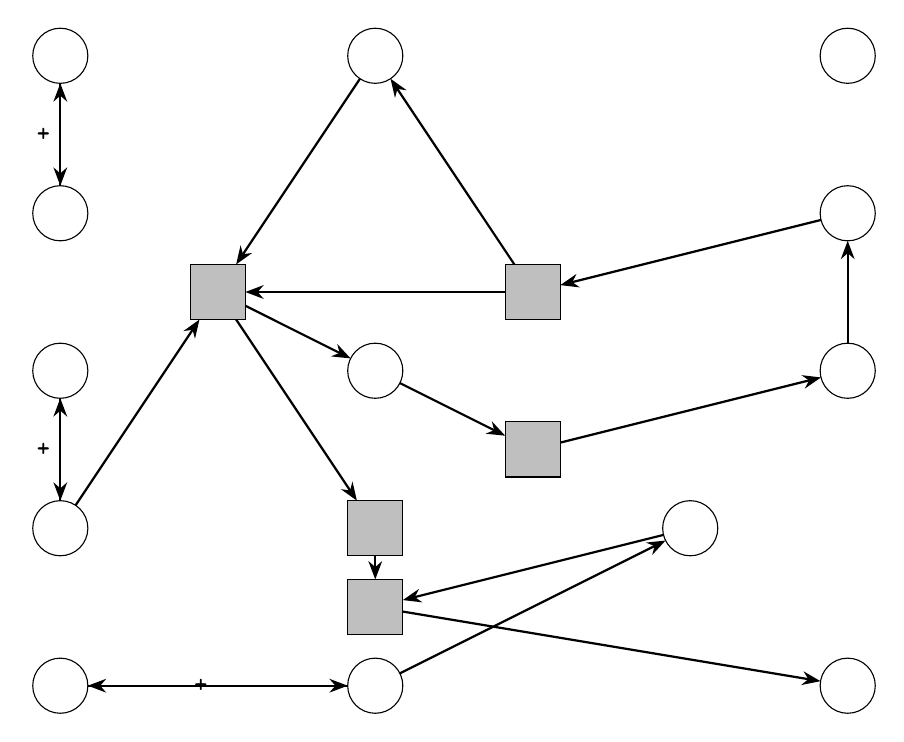
\begin{tikzpicture}[node distance=1.5cm, auto]

% Define places
\node[place, label=above:{Glucagon}] (glucagon) at (-4, 4) {};
\node[place, label=above:{Glucose}] (glucose) at (0, 4) {};
\node[place, label=above:{Insulin}] (insulin) at (6, 4) {};
\node[place, label=left:{cAMP}] (camp) at (-4, 2) {};
\node[place, label=left:{PXA}] (pxa) at (-4, 0) {};
\node[place, label=below left:{nSFP51}] (nsfp51) at (-4, -2) {};
\node[place, label=below left:{Pho}] (pho) at (-4, -4) {};
\node[place, label=right:{GK}] (gk) at (6, 2) {};
\node[place, label=right:{PP}] (pp) at (6, 0) {};
\node[place, label=right:{Kin}] (kin) at (6, -4) {};
\node[place, label=below right:{mF26P2}] (mf26p2) at (0, -4) {};
\node[place, label=above:{Pyruvate}] (pyruvate) at (0, 0) {};
\node[place, label=above right:{InfBPase}] (infbpase) at (4, -2) {};

% Define transitions
\node[transition, label=below:{a6PFK1}] (a6pfk1) at (-2, 1) {};
\node[transition, label=below:{aFBPase}] (afbpase) at (2, 1) {};
\node[transition, label=below:{I-FBPase}] (ifbpase) at (2, -1) {};
\node[transition, label=below:{F26P2}] (f26p2) at (0, -2) {};
\node[transition, label=below:{mF26P2}] (mf26p2_trans) at (0, -3) {};

% Draw arcs (arrows)
\draw[arrow] (glucagon) -- node[left]{\small \texttt{+}} (camp);
\draw[arrow] (camp) -- node[left]{\small \texttt{-}} (glucagon);
\draw[arrow] (pxa) -- node[left]{\small \texttt{+}} (nsfp51);
\draw[arrow] (nsfp51) -- node[left]{\small \texttt{-}} (pxa);
\draw[arrow] (pho) -- node[left]{\small \texttt{+}} (mf26p2);
\draw[arrow] (mf26p2) -- node[left]{\small \texttt{-}} (pho);

\draw[arrow] (glucose) -- (a6pfk1);
\draw[arrow] (gk) -- (afbpase);
\draw[arrow] (afbpase) -- (glucose);
\draw[arrow] (a6pfk1) -- (pyruvate);
\draw[arrow] (pyruvate) -- (ifbpase);
\draw[arrow] (ifbpase) -- (pp);
\draw[arrow] (pp) -- (gk);

\draw[arrow] (nsfp51) -- (a6pfk1);
\draw[arrow] (afbpase) -- (a6pfk1);
\draw[arrow] (a6pfk1) -- (f26p2);
\draw[arrow] (f26p2) -- (mf26p2_trans);
\draw[arrow] (mf26p2_trans) -- (kin);
\draw[arrow] (infbpase) -- (mf26p2_trans);
\draw[arrow] (mf26p2) -- (infbpase);

\end{tikzpicture}

\end{document}